\documentclass[varwidth=true, border=2pt]{standalone}
\usepackage{tkz-euclide}

\begin{document}
\usetkzobj{all}
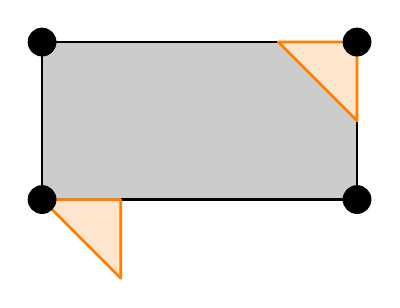
\begin{tikzpicture}
    \tkzSetUpPoint[shape=circle,size=10,color=black,fill=black]
    \tkzSetUpLine[line width=1]
    \tkzDefPoints{0/0/A, 4/0/B, 4/2/C, 0/2/D, 3/2/E, 4/1/F, 1/0/G, 1/-1/H}
    \tkzDrawPolygon[fill=black!20](A,B,C,D)
    \tkzDrawPolygon[orange,fill=orange!20](E,C,F)
    \tkzDrawPolygon[orange,fill=orange!20](A,G,H)
    \tkzDrawPoints(A,B,C,D)
\end{tikzpicture}
\end{document}
